\begin{frame}
    \frametitle{Analytical formulation - M|M|1 queue}
    \centering

    % DES Diagram
    \begin{tikzpicture}[>=stealth, scale=0.8] 
        \draw (2,1.25) -- ++(5cm,0) -- ++(0,-1.5cm) -- ++(-5cm,0);
        \foreach \i in {1,...,6}
        \draw (7cm-\i*15pt,1.25) -- +(0,-1.5cm);
        \draw (7.9,0.5) circle [radius=0.75cm];
        \node[] at (0.7, 0.55) {$\lambda$};
        \draw[->] (1, 0.525) -- (2.1, 0.525);
        \draw[->] (8.7,0.525) -- +(20pt,0);
        \only<1>{
            \node[] at (7.9,0.5) {$\mu$};
        }
        \only<2,3,4>{            
            \node[blue] at (0.7, 0.55) {$\lambda$};
            \draw[->, blue] (1, 0.525) -- (2.1, 0.525);
        }
        \only<2,3,4,5>{
            \node[draw=none, blue] at (7.9,0.5) {\Large{\Strichmaxerl[1]}};
        }
        \only<3,4,5>{
            \node[draw=none, blue] at (6.74,0.5) {\Large{\Strichmaxerl[1]}};
        }
        \only<4>{
            \node[draw=none, blue] at (6.2,0.5) {\Large{\Strichmaxerl[1]}};
        }
        \only<5>{
            \draw[->, blue] (8.7,0.525) -- +(20pt,0);
        }
    \end{tikzpicture}

    \vspace{0.6cm}

    % Markov Chain
    \begin{tikzpicture}[-, node distance = 0.7cm, auto, every node/.style={scale=0.5}]
        \node[state] (one) {0};
        \node[state, right=of one] (two) {1};
        \node[state, right=of two] (three) {2};
        \node[state, right=of three] (four) {3};
        \node[state, right=of four] (five) {4};
        \node[state, right=of five] (six) {5};
        \node[state, right=of six] (seven) {6};

        \draw[every loop]
            (one) edge[bend left] node {\( \lambda \)} (two)
            (two) edge[bend left] node {\( \mu \)} (one)
            (two) edge[bend left] node {\( \lambda \)} (three)
            (three) edge[bend left] node {\( \mu \)} (two)
            (three) edge[bend left] node {\( \lambda \)} (four)
            (four) edge[bend left] node {\( \mu \)} (three)
            (four) edge[bend left] node {\( \lambda \)} (five)
            (five) edge[bend left] node {\( \mu \)} (four)
            (five) edge[bend left] node {\( \lambda \)} (six)
            (six) edge[bend left] node {\( \mu \)} (five)
            (six) edge[bend left] node {\( \lambda \)} (seven)
            (seven) edge[bend left] node {\( \mu \)} (six)
            ;

        \only<1>{\node[state, ultra thick] (one) {0};}
        \only<2>{
            \node[state, blue, ultra thick, right=of one] (two) {1};
            \draw[every loop, blue] (one) edge[bend left] node {\( \lambda \)} (two);
        }
        \only<3>{
            \node[state, blue, ultra thick, right=of two] (three) {2};
            \draw[every loop, blue] (two) edge[bend left] node {\( \lambda \)} (three);
        }
        \only<4>{
            \node[state, blue, ultra thick, right=of three] (four) {3};
            \draw[every loop, blue] (three) edge[bend left] node {\( \lambda \)} (four);
        }
        \only<5>{
            \node[state, blue, ultra thick, left=of four] (three) {2};
            \draw[every loop, blue] (four) edge[bend left] node {\( \mu \)} (three);
        }
    \end{tikzpicture}

    % Generator Matrix
    \tiny
    \begin{equation*}
        Q = 
        \begin{blockarray}{cccccccc}
            (0) & (1) & (2) & (3) & (4) & (5) & (6) &\\
            & & & & & & & & \\
            \begin{block}{(ccccccc)c}
                -\lambda & \lambda & 0 & 0 & 0 & 0 & 0 & (0) \\
                \mu & -\mu - \lambda & \lambda & 0 & 0 & 0 & 0 & (1) \\
                0 & \mu & -\mu - \lambda & \lambda & 0 & 0 & 0 & (2) \\
                0 & 0 & \mu & -\mu - \lambda & \lambda & 0 & 0 & (3) \\
                0 & 0 & 0 & \mu & -\mu - \lambda & \lambda & 0 & (4) \\
                0 & 0 & 0 & 0 & \mu & -\mu - \lambda & \lambda & (5) \\
                0 & 0 & 0 & 0 & 0 & \mu & -\mu & (6) \\
            \end{block}
        \end{blockarray}    
    \end{equation*}
    \normalsize
\end{frame}


\begin{frame}
    \frametitle{Analytical formulation - M|M|3 queue}
    \centering

    \begin{tikzpicture}[-, node distance = 0.8cm, auto, every node/.style={scale=0.6}]
        \node[state] (one) {0};
        \node[state, right=of one] (two) {1};
        \node[state, right=of two] (three) {2};
        \node[state, right=of three] (four) {3};
        \node[state, right=of four] (five) {4};
        \node[state, right=of five] (six) {5};
        \node[state, right=of six] (seven) {6};

        \draw[every loop]
            (one) edge[bend left] node {\( \lambda \)} (two)
            (two) edge[bend left] node {\( \mu \)} (one)
            (two) edge[bend left] node {\( \lambda \)} (three)
            (three) edge[bend left] node {\( 2\mu \)} (two)
            (three) edge[bend left] node {\( \lambda \)} (four)
            (four) edge[bend left] node {\( 3\mu \)} (three)
            (four) edge[bend left] node {\( \lambda \)} (five)
            (five) edge[bend left] node {\( 3\mu \)} (four)
            (five) edge[bend left] node {\( \lambda \)} (six)
            (six) edge[bend left] node {\( 3\mu \)} (five)
            (six) edge[bend left] node {\( \lambda \)} (seven)
            (seven) edge[bend left] node {\( 3\mu \)} (six)
            ;
    \end{tikzpicture}

    \vspace{0.6cm}

    % Generator Matrix
    \scriptsize
    \begin{equation*}
        Q = 
        \begin{blockarray}{cccccccc}
            (0) & (1) & (2) & (3) & (4) & (5) & (6) &\\
            & & & & & & & & \\
            \begin{block}{(ccccccc)c}
                -\lambda & \lambda & 0 & 0 & 0 & 0 & 0 & (0) \\
                \mu & -\mu - \lambda & \lambda & 0 & 0 & 0 & 0 & (1) \\
                0 & 2\mu & -2\mu - \lambda & \lambda & 0 & 0 & 0 & (2) \\
                0 & 0 & 3\mu & -3\mu - \lambda & \lambda & 0 & 0 & (3) \\
                0 & 0 & 0 & 3\mu & -3\mu - \lambda & \lambda & 0 & (4) \\
                0 & 0 & 0 & 0 & 3\mu & -3\mu - \lambda & \lambda & (5) \\
                0 & 0 & 0 & 0 & 0 & 3\mu & -3\mu & (6) \\
            \end{block}
        \end{blockarray}    
    \end{equation*}
            
\end{frame}


\begin{frame}
    \frametitle{Analytical formulation - Custom Queue}
    \centering

    \begin{tikzpicture}[>=stealth, scale=0.6] %arrow type
        % the rectangle with vertical rules (Queue 1)
        \draw (0,0) -- ++(2cm,0) -- ++(0,-1.5cm) -- ++(-2cm,0);
        \foreach \i in {1,...,3, 3.8}
        \draw (2cm-\i*15pt,0) -- +(0,-1.5cm);
        
        % the circle (Queue 1)
        \draw (2.75,-0.75cm) circle [radius=0.75cm];

        % the rectangle with vertical rules (Queue 2)
        \draw (5,1.25) -- ++(2cm,0) -- ++(0,-1.5cm) -- ++(-2cm,0);
        \foreach \i in {1,...,4, 5.7}
        \draw (7cm-\i*10pt,1.25) -- +(0,-1.5cm);

        % The two vertical lines at the very start of Queue 2 
        \draw (7cm-54pt,1.2) -- +(0,-0.5cm);
        \draw (7cm-54pt,0.3) -- +(0,-0.5cm);        
        \draw (7cm-51pt,1.1) -- +(0,-0.4cm);
        \draw (7cm-51pt,0.3) -- +(0,-0.4cm);

        % The label between the lines for T
        \node[anchor=north] at (5.12, 0.85 cm) {\tiny{\( T \)}};

        % the circle (Queue 2)
        \draw (7.75,0.5) circle [radius=0.75cm];

        % the arrows and labels (Queue 1+2)
        \draw[->] (8.5,0.525) -- +(20pt,0);
        \node[align=center] at (1cm,-2cm) {};
        \node[align=center] at (2.75cm,-2cm) {Parking};
        \node[align=center] at (6cm,-0.75cm) {};
        \node[align=center] at (7.8cm,-0.75cm) {Hospital};
        
        % Ambulance lines
        \draw[<-] (0,-0.75) -- +(-50pt,0) node[left] {\( \lambda_2 \)};
        \draw[-] (3.5,-0.75) -- +(20pt,0);
        \draw (4.2, 0.525) -- (4.2, -0.75);

        % Others lines
        \draw (4.2, 1.8) -- +(-169.5pt,0) node[left] {\( \lambda_1 \)};
        \draw (4.2, 1.8) -- (4.2, 0.525);
        \draw[->] (4.2, 0.525) -- (5, 0.525);


        % Animations
        \only<2,3,4,5,6>{
            \node[draw=none, red] at (7.5,0.75) {\Strichmaxerl[1]};
        }
        \only<3,4,5,6>{
            \node[draw=none, blue] at (8,0.75) {\Strichmaxerl[1]};
        }
        \only<4,5,6>{
            \node[draw=none, red] at (7.75,0.25) {\Strichmaxerl[1]};
        }
        \only<2,4>{
            \draw[red, very thick] (4.2, 1.8) -- +(-169.5pt,0) node[left] {\( \lambda_1 \)};
            \draw[red, very thick] (4.2, 1.8) -- (4.2, 0.525);
            \draw[->, red, very thick] (4.2, 0.525) -- (5, 0.525);
        }
        \only<3>{
            \draw[<-, blue, very thick] (0,-0.75) -- +(-50pt,0) node[left] {\( \lambda_2 \)};
            \draw[-, blue, very thick] (3.5,-0.75) -- +(20pt,0);
            \draw[blue, very thick] (4.2, 0.525) -- (4.2, -0.75);
            \draw[->, blue, very thick] (4.2, 0.525) -- (5, 0.525);
        }
        \only<5,6>{
            \draw[<-, blue, very thick] (0,-0.75) -- +(-50pt,0) node[left] {\( \lambda_2 \)};
            \node[draw=none, blue] at (2.75,-0.75) {\Strichmaxerl[1]};
        }
        \only<6>{
            % \draw[blue, very thick] (2cm-10pt,0) -- +(0,-1.5cm);
            \node[draw=none, blue] at (1.72,-0.75) {\Strichmaxerl[1]};
        }
    \end{tikzpicture}

    \begin{figure}
        \begin{tikzpicture}[-, node distance = 0.7cm, auto, every node/.style={scale=0.5}]
            \only<1,2,3,4,5,6>{
                \node[state] (one) {(0,0)};
                \node[state, right=of one] (two) {(0,1)};
                \node[state, right=of two] (three) {(0,2)};
                \node[state, right=of three] (four) {(0,3)};
                \node[state, right=of four] (five) {(0,4)};
                \node[state, below=of three] (three_one) {(1,2)};
                \node[state, below=of three_one] (three_two) {(2,2)};
                \node[state, below=of four] (four_one) {(1,3)};
                \node[state, below=of four_one] (four_two) {(2,3)};
                \node[state, below=of five] (five_one) {(1,4)};
                \node[state, below=of five_one] (five_two) {(2,4)};
                \draw[every loop]
                    (one) edge[bend left] node {\( \lambda_1 + \lambda_2 \)} (two)
                    (two) edge[bend left] node {\( \mu \)} (one)
                    (two) edge[bend left] node {\( \lambda_1 + \lambda_2 \)} (three)
                    (three) edge[bend left] node {\( 2\mu \)} (two)
                    (three) edge[bend left] node {\( \lambda_1 \)} (four)
                    (four) edge[bend left] node {\( 3\mu \)} (three)
                    (four) edge[bend left] node {\( \lambda_1 \)} (five)
                    (five) edge[bend left] node {\( 3\mu \)} (four)
                    (three) edge[bend left] node {\( \lambda_2 \)} (three_one)
                    (three_one) edge[bend left] node {\( 2\mu \)} (three)
                    (three_one) edge[bend left] node {\( \lambda_1 \)} (four_one)
                    (four_one) edge[bend left] node {\( 3\mu \)} (three_one)
                    (four_one) edge[bend left] node {\( \lambda_1 \)} (five_one)
                    (five_one) edge[bend left] node {\( 3\mu \)} (four_one)
                    (four) edge node {\( \lambda_2 \)} (four_one)
                    (five) edge node {\( \lambda_2 \)} (five_one)
                    (three_one) edge[bend left] node {\( \lambda_2 \)} (three_two)
                    (three_two) edge[bend left] node {\( 2\mu \)} (three_one)
                    (four_one) edge node {\( \lambda_2 \)} (four_two)
                    (five_one) edge node {\( \lambda_2 \)} (five_two)
                    (three_two) edge[bend left] node {\( \lambda_1 \)} (four_two)
                    (four_two) edge[bend left] node {\( 3\mu \)} (three_two)
                    (four_two) edge[bend left] node {\( \lambda_1 \)} (five_two)
                    (five_two) edge[bend left] node {\( 3\mu \)} (four_two)
                    ;
            }
            \only<1>{\node[state, ultra thick] (one) {(0,0)};}
            \only<2>{
                \node[state, ultra thick, red, right=of one] (two) {(0,1)};
                \draw[every loop, red] (one) edge[bend left] node {\( \lambda_1 + \lambda_2 \)} (two);
            }
            \only<3>{
                \node[state, ultra thick, blue, right=of two] (three) {(0,2)};
                \draw[every loop, blue] (two) edge[bend left] node {\( \lambda_1 + \lambda_2 \)} (three);
            }
            \only<4>{
                \node[state, ultra thick, red, right=of three] (four) {(0,3)};
                \draw[every loop, red] (three) edge[bend left] node {\( \lambda_1 \)} (four);
            }
            \only<5>{
                \node[state, ultra thick, blue, below=of four] (four_one) {(1,3)};
                \draw[every loop, blue] (four) edge node {\( \lambda_2 \)} (four_one);
            }
            \only<6>{
                \node[state, ultra thick, blue, below=of four_one] (four_two) {(2,3)};
                \draw[every loop, blue] (four_one) edge node {\( \lambda_2 \)} (four_two);
            }
        \end{tikzpicture}
    \end{figure}
\end{frame}



\begin{frame}
    \frametitle{Analytical formulation - Custom Queue}
    \centering

    \tiny
    \begin{tikzpicture}[-, node distance = 0.6cm, auto, every node/.style={scale=0.9}]
        \node[state] (one) {(0,0)};
        \node[state, right=of one] (two) {(0,1)};
        \node[state, right=of two] (three) {(0,2)};
        \node[state, right=of three] (four) {(0,3)};
        \node[state, right=of four] (five) {(0,4)};
        \node[state, below=of three] (three_one) {(1,2)};
        \node[state, below=of three_one] (three_two) {(2,2)};
        \node[state, below=of four] (four_one) {(1,3)};
        \node[state, below=of four_one] (four_two) {(2,3)};
        \node[state, below=of five] (five_one) {(1,4)};
        \node[state, below=of five_one] (five_two) {(2,4)};
        \draw[every loop]
            (one) edge[bend left] node {\( \lambda_1 + \lambda_2 \)} (two)
            (two) edge[bend left] node {\( \mu \)} (one)
            (two) edge[bend left] node {\( \lambda_1 + \lambda_2 \)} (three)
            (three) edge[bend left] node {\( 2\mu \)} (two)
            (three) edge[bend left] node {\( \lambda_1 \)} (four)
            (four) edge[bend left] node {\( 3\mu \)} (three)
            (four) edge[bend left] node {\( \lambda_1 \)} (five)
            (five) edge[bend left] node {\( 3\mu \)} (four)
            (three) edge[bend left] node {\( \lambda_2 \)} (three_one)
            (three_one) edge[bend left] node {\( 2\mu \)} (three)
            (three_one) edge[bend left] node {\( \lambda_1 \)} (four_one)
            (four_one) edge[bend left] node {\( 3\mu \)} (three_one)
            (four_one) edge[bend left] node {\( \lambda_1 \)} (five_one)
            (five_one) edge[bend left] node {\( 3\mu \)} (four_one)
            (four) edge node {\( \lambda_2 \)} (four_one)
            (five) edge node {\( \lambda_2 \)} (five_one)
            (three_one) edge[bend left] node {\( \lambda_2 \)} (three_two)
            (three_two) edge[bend left] node {\( 2\mu \)} (three_one)
            (four_one) edge node {\( \lambda_2 \)} (four_two)
            (five_one) edge node {\( \lambda_2 \)} (five_two)
            (three_two) edge[bend left] node {\( \lambda_1 \)} (four_two)
            (four_two) edge[bend left] node {\( 3\mu \)} (three_two)
            (four_two) edge[bend left] node {\( \lambda_1 \)} (five_two)
            (five_two) edge[bend left] node {\( 3\mu \)} (four_two)
            ;
    \end{tikzpicture}

    \begin{equation*}
        Q = 
        \begin{blockarray}{cccccccc}
            (0, 0) & (0, 1) & (0, 2) & & (2, 3) & (2, 4) & & \\
            & & & & & & & &\\
            \begin{block}{(cccccc)cc}
                -\lambda_1 - \lambda_2 & \lambda_1 + \lambda_2 & 0 & \dots & 0 & 0 & & (0,0) \\
                \mu & -\mu - \lambda_1 - \lambda_2 & \lambda_1 + \lambda_2 & \dots & 0 & 0 & & (0,1) \\
                0 & 2\mu & -2\mu - \lambda_1 - \lambda_2 & \dots & 0 & 0 & & (0,2) \\
                \vdots & \vdots & \vdots & \ddots & \vdots & \vdots & \\
                0 & 0 & 0 & \dots & -\lambda_1 - 3\mu & \lambda_1 & & (2,3)\\
                0 & 0 & 0 & \dots & 3\mu & -3\mu & & (2,4) \\
            \end{block}
        \end{blockarray}    
    \end{equation*}

\end{frame}
